% AI-assisted code: generated and revised with Claude Opus 5.5
% under the author's direction; reviewed and tested by the author
% (see the thesis section "Use of AI tools").
% UML class diagram of the core domain (matches src/evoalgo at commit 7895107).
% Layout: Orchestrator in the centre; domain model left, verification right,
% agents below, persistence/eventing in a bottom row.
\documentclass[border=4pt]{standalone}
% Shared TikZ style for the thesis UML figures (standalone documents).
\usepackage[T1]{fontenc}
\usepackage{lmodern}
\usepackage{tikz}
\usetikzlibrary{positioning,arrows.meta,shapes.multipart,shapes.geometric,fit,backgrounds,calc,matrix}
\definecolor{umlfill}{HTML}{F4F6FA}
\definecolor{umlline}{HTML}{3A4150}
\definecolor{umlaccent}{HTML}{0071E3}
\tikzset{
  every node/.style={font=\sffamily\small},
  % class box: \node[class] {Name \nodepart{second} attrs \nodepart{third} ops};
  class/.style={rectangle split, rectangle split parts=3, draw=umlline, fill=umlfill,
    align=left, rectangle split part align={center,left,left}, inner sep=3pt, font=\sffamily\scriptsize},
  % generalisation (hollow triangle), realisation (dashed, hollow triangle)
  inherit/.style={-{Triangle[open,length=7pt,width=7pt]}, draw=umlline},
  realize/.style={-{Triangle[open,length=7pt,width=7pt]}, dashed, draw=umlline},
  % composition (filled diamond at the whole), aggregation (hollow), association, dependency
  compose/.style={{Diamond[length=9pt,width=6pt]}-, draw=umlline},
  aggregate/.style={{Diamond[open,length=9pt,width=6pt]}-, draw=umlline},
  assoc/.style={-, draw=umlline},
  navassoc/.style={-{Straight Barb[length=5pt]}, draw=umlline},
  depend/.style={-{Straight Barb[length=5pt]}, dashed, draw=umlline},
  mult/.style={font=\sffamily\tiny, inner sep=1pt},
  stereo/.style={font=\sffamily\tiny\itshape},
}

\begin{document}
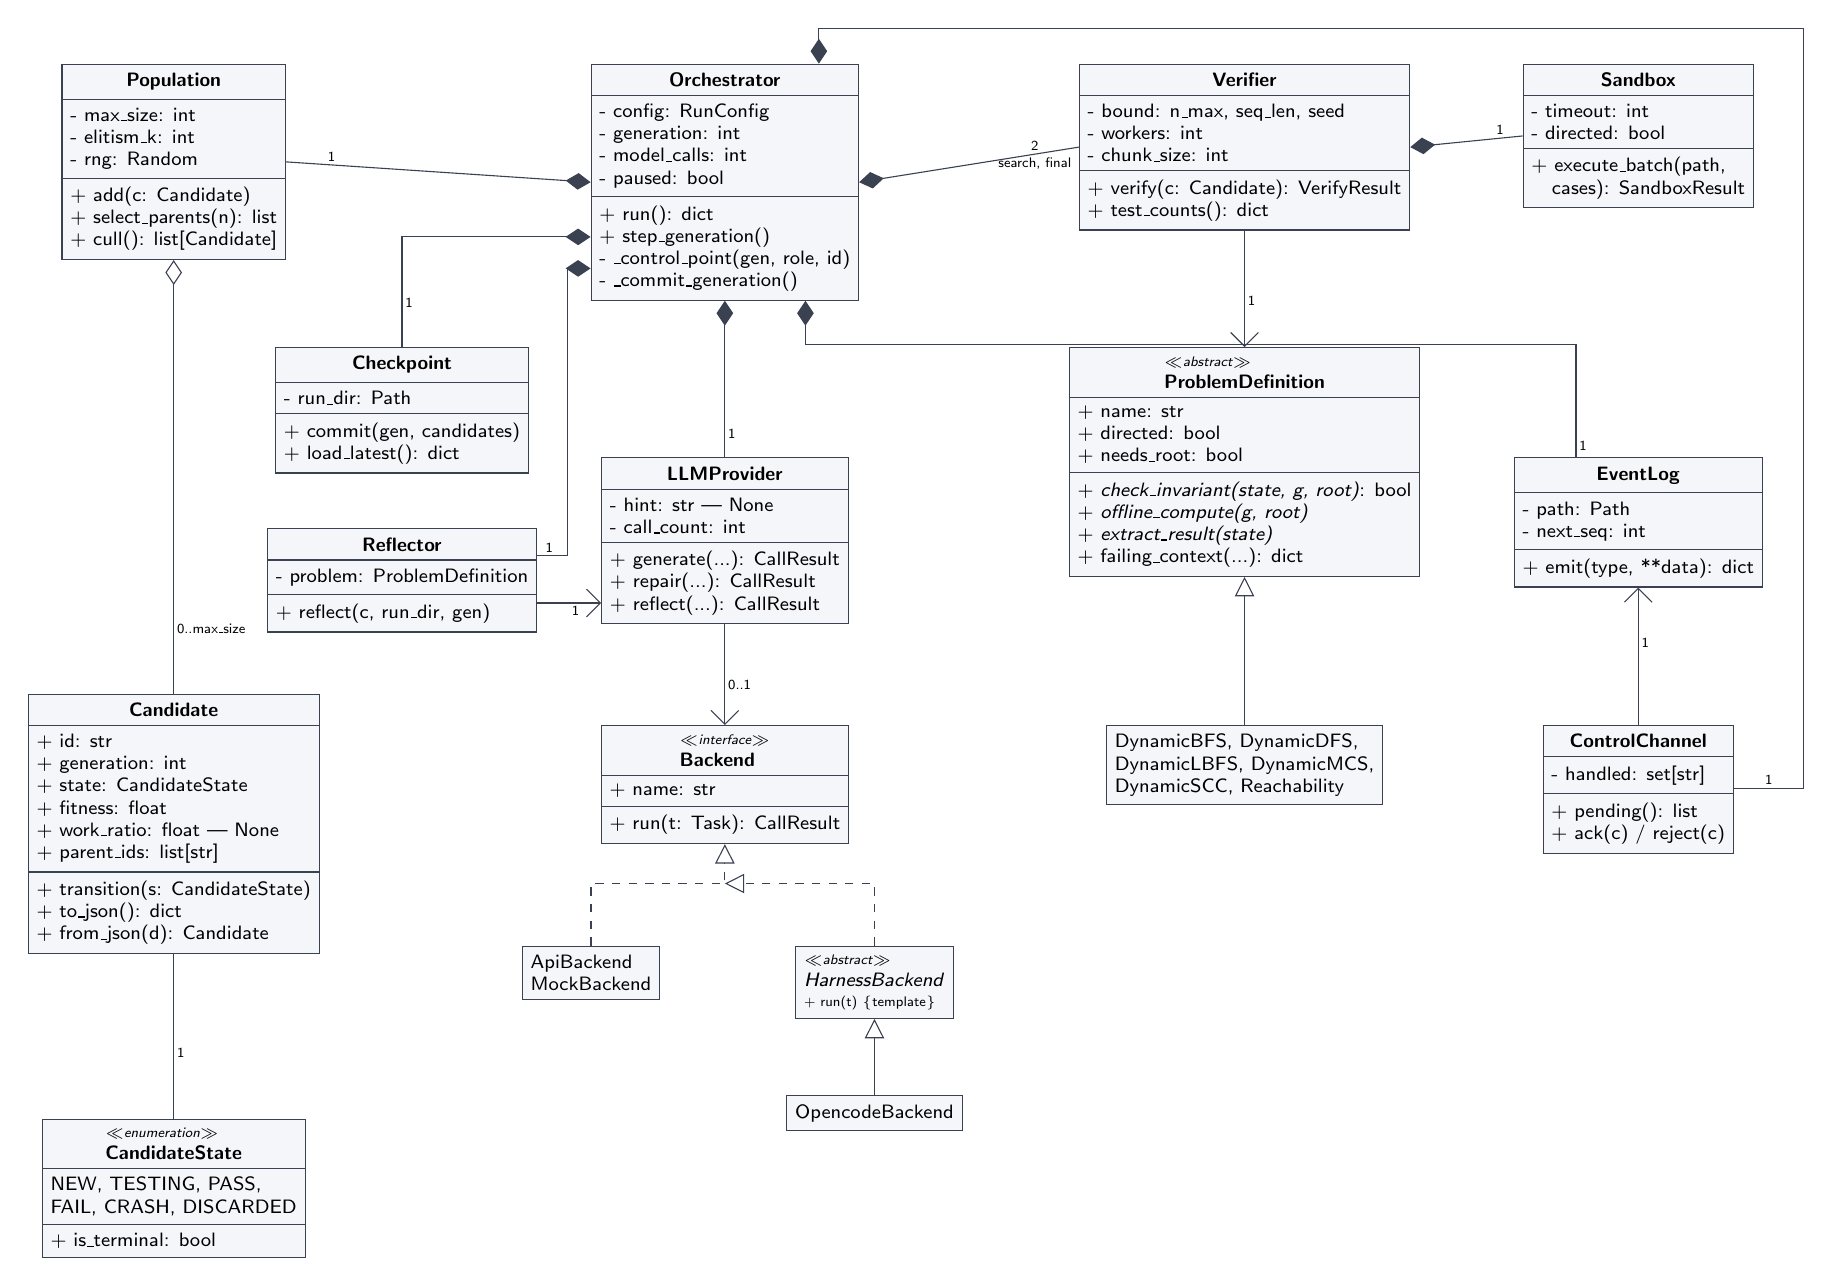
\begin{tikzpicture}
  % ------------------------------------------------------------ centre column
  \node[class, anchor=north] (orch) at (7,0) {\textbf{Orchestrator}
    \nodepart{second} - config: RunConfig\\ - generation: int\\ - model\_calls: int\\ - paused: bool
    \nodepart{third} + run(): dict\\ + step\_generation()\\ - \_control\_point(gen, role, id)\\ - \_commit\_generation()};
  \node[class, anchor=north] (llm) at (7,-5.0) {\textbf{LLMProvider}
    \nodepart{second} - hint: str | None\\ - call\_count: int
    \nodepart{third} + generate(...): CallResult\\ + repair(...): CallResult\\ + reflect(...): CallResult};
  \node[class, anchor=north] (backend) at (7,-8.4) {{\tiny\itshape$\ll$interface$\gg$}\\\textbf{Backend}
    \nodepart{second} + name: str
    \nodepart{third} + run(t: Task): CallResult};
  \node[class, rectangle split parts=1, anchor=north] (backs) at (5.3,-11.2) {ApiBackend\\ MockBackend};
  \node[class, rectangle split parts=1, anchor=north] (hb) at (8.9,-11.2) {{\tiny\itshape$\ll$abstract$\gg$}\\\textit{HarnessBackend}\\[-1pt]{\tiny + run(t) \{template\}}};
  \node[class, rectangle split parts=1, anchor=north] (harn) at (8.9,-13.1) {OpencodeBackend};
  \node[class, anchor=north] (refl) at (2.9,-5.9) {\textbf{Reflector}
    \nodepart{second} - problem: ProblemDefinition
    \nodepart{third} + reflect(c, run\_dir, gen)};
  % ------------------------------------------------------------- left column
  \node[class, anchor=north] (pop) at (0,0) {\textbf{Population}
    \nodepart{second} - max\_size: int\\ - elitism\_k: int\\ - rng: Random
    \nodepart{third} + add(c: Candidate)\\ + select\_parents(n): list\\ + cull(): list[Candidate]};
  \node[class, anchor=north] (cand) at (0,-8.0) {\textbf{Candidate}
    \nodepart{second} + id: str\\ + generation: int\\ + state: CandidateState\\ + fitness: float\\ + work\_ratio: float | None\\ + parent\_ids: list[str]
    \nodepart{third} + transition(s: CandidateState)\\ + to\_json(): dict\\ + from\_json(d): Candidate};
  \node[class, anchor=north] (state) at (0,-13.4) {{\tiny\itshape$\ll$enumeration$\gg$}\\\textbf{CandidateState}
    \nodepart{second} NEW, TESTING, PASS,\\ FAIL, CRASH, DISCARDED
    \nodepart{third} + is\_terminal: bool};
  % ------------------------------------------------------------ right column
  \node[class, anchor=north] (ver) at (13.6,0) {\textbf{Verifier}
    \nodepart{second} - bound: n\_max, seq\_len, seed\\ - workers: int\\ - chunk\_size: int
    \nodepart{third} + verify(c: Candidate): VerifyResult\\ + test\_counts(): dict};
  \node[class, anchor=north] (sb) at (18.6,0) {\textbf{Sandbox}
    \nodepart{second} - timeout: int\\ - directed: bool
    \nodepart{third} + execute\_batch(path,\\ \quad cases): SandboxResult};
  \node[class, anchor=north] (pd) at (13.6,-3.6) {{\tiny\itshape$\ll$abstract$\gg$}\\\textbf{\textit{ProblemDefinition}}
    \nodepart{second} + name: str\\ + directed: bool\\ + needs\_root: bool
    \nodepart{third} + \textit{check\_invariant(state, g, root)}: bool\\ + \textit{offline\_compute(g, root)}\\ + \textit{extract\_result(state)}\\ + failing\_context(...): dict};
  \node[class, rectangle split parts=1, anchor=north] (sub) at (13.6,-8.4) {DynamicBFS, DynamicDFS,\\ DynamicLBFS, DynamicMCS,\\ DynamicSCC, Reachability};
  % ------------------------------------------------- persistence / eventing
  \node[class, anchor=north] (ck) at (2.9,-3.6) {\textbf{Checkpoint}
    \nodepart{second} - run\_dir: Path
    \nodepart{third} + commit(gen, candidates)\\ + load\_latest(): dict};
  \node[class, anchor=north] (log) at (18.6,-5.0) {\textbf{EventLog}
    \nodepart{second} - path: Path\\ - next\_seq: int
    \nodepart{third} + emit(type, **data): dict};
  \node[class, anchor=north] (ctl) at (18.6,-8.4) {\textbf{ControlChannel}
    \nodepart{second} - handled: set[str]
    \nodepart{third} + pending(): list\\ + ack(c) / reject(c)};

  % --------------------------------------------------------------- relations
  % The Orchestrator owns ...
  \draw[compose] (orch.west) -- node[mult, above, pos=0.85] {1} (pop.east);
  \draw[compose] (orch.east) -- node[mult, above, pos=0.8] {2} node[mult, below, pos=0.8] {search, final} (ver.west);
  \draw[compose] (orch.south) -- node[mult, right, pos=0.85] {1} (llm.north);
  % Checkpoint and Reflector: from the Orchestrator's west edge (measured box edges:
  % Orchestrator x 5.21..8.79, LLMProvider from x 5.43, Reflector/Checkpoint up to x 4.61).
  \draw[compose] (orch.west|-0,-2.2) -- (2.9,-2.2) -- node[mult, right, pos=0.6] {1} (ck.north);
  \draw[compose] (orch.west|-0,-2.6) -- (5.0,-2.6) -- (5.0,-6.25) -- node[mult, above, pos=0.6] {1} (refl.east|-0,-6.25);
  \draw[compose] ($(orch.south east)!0.4!(orch.south)$) -- ++(0,-0.55) -| node[mult, right, pos=0.95] {1} ($(log.north west)!0.5!(log.north)$);
  % domain model
  \draw[aggregate] (pop.south) -- node[mult, right, pos=0.85] {0..max\_size} (cand.north);
  \draw[assoc] (cand.south) -- node[mult, right, pos=0.6] {1} (state.north);
  % verification
  \draw[compose] (ver.east) -- node[mult, above, pos=0.8] {1} (sb.west);
  \draw[navassoc] (ver.south) -- node[mult, right, pos=0.6] {1} (pd.north);
  \draw[inherit] (sub.north) -- (pd.south);
  % agents
  \draw[navassoc] (refl.east|-0,-6.85) -- node[mult, below, pos=0.6] {1} (llm.west|-0,-6.85);
  \draw[navassoc] (llm.south) -- node[mult, right, pos=0.6] {0..1} (backend.north);
  \draw[realize] (backs.north) |- ($(backend.south)+(0,-0.5)$) -- (backend.south);
  \draw[realize] (hb.north) |- ($(backend.south)+(0,-0.5)$);
  \draw[inherit] (harn.north) -- (hb.south);
  % eventing
  % ControlChannel uses the Orchestrator's EventLog (passed in), it does not own it.
  \draw[navassoc] (ctl.north) -- node[mult, right, pos=0.6] {1} (log.south);
  % The Orchestrator owns the ControlChannel (orchestrator.py: self.control).
  % Routed over the top and down the right margin (measured: Verifier/Sandbox tops at
  % y 0, right column x up to 20.18), so it crosses no box and no other edge.
  \draw[compose] ($(orch.north east)!0.3!(orch.north)$) -- ++(0,0.45) -- (20.7,0.45) -- (20.7,-9.2)
    -- node[mult, above, pos=0.5] {1} (ctl.east|-0,-9.2);
\end{tikzpicture}
\end{document}
